\documentclass{beamer}
\usetheme{metropolis}
\usepackage{polski}    
\usepackage[]{listings}       % Use metropolis theme
\title{Praca na zaliczenie przemiotu: Zastosowanie zaawansowanych narzędzi arkusza kalkulacyjnego i kodów komputerowych w zagadnieniach matematyki i analizy danych}
\date{\today}
\author{Julia Czachor, Krystian Oleniacz}
\begin{document}
  \maketitle
  \begin{frame}{Analiza danych}
    Do analizy wybrane zostały ceny akcji spółek Visa i Mastercard z lat 2019-2022. 
  \end{frame}
  \begin{frame}{Optymalizacja}
    Rozwiązane zadanie 75 ze strony 108 książki Badania operacyjne w przykładach 
    i zadaniach pod redakcją Karola Kukuły. 

    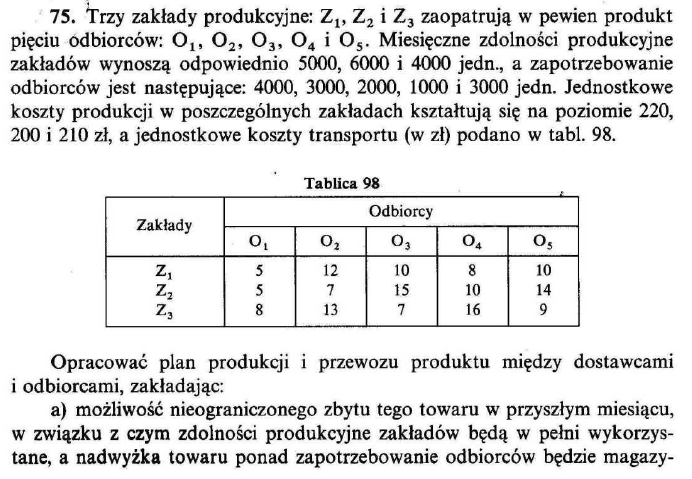
\includegraphics[scale=0.5]{images/obrazek1.png}
    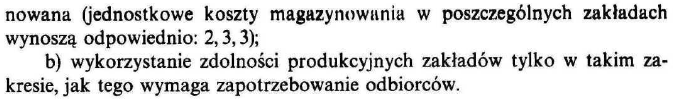
\includegraphics[scale=0.5]{images/obrazek2.png}
  \end{frame}
  \begin{frame}{Optymalizacja}
    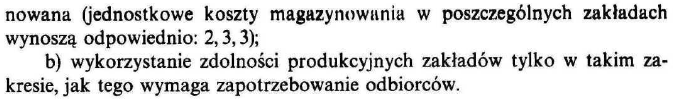
\includegraphics[scale=0.5]{images/obrazek2.png}
  \end{frame}
 
  \begin{frame}{Prawdopodobieństwo}
    Danych jest 5 pudełek ponumerowanych liczbami od 1 do 5. W każdym pudełku znajduje się 20 kul ponumerowanych liczbami od 1 do 20.
    Z każdego pudełka wybieramy jedną kulę. Oblicz prawdopodobieństwo zdarzenia polegającego na tym, że każda z wylosowanych liczb jest
    mniejsza od wszystkich liczb wylosowanych z pudełek o większych numerach oraz suma wylosowanych liczb jest podzielna przez 3.  
    \end{frame}

  
\end{document}